\chapter{Projeto - Parte 4}\label{ch:projeto-parte4}


\section{Arquitetura Deliberativa}\label{sec:arquitetura-deliberativa}

Conforme foi abordado na secção~\ref{sec:arquiteturas-reativa-memoria}, um agente reativo com memória age com conhecimento do presente, através de reações a estímulos, e com conhecimento do passado, através da memorização de percepções e de ações passadas.
Já um agente com uma arquitetura deliberativa, para além de ter o conhecimento que um agente reativo apresenta, tem a capacidade de antecipar o futuro, através da simulação de cenários, e de tomar decisões com base nessa antecipação.

Na arquitetura deliberativa, o agente é composto por três componentes~\cite{isel:iasa:slides:arq-agentes-deliberativos}:

Na arquitectura deliberativa, a memória é o componente que desempenha um papel central na geração do comportamento do agente.
É através da memória que o agente tem a capacidade de representar o mundo e os mecanismos de deliberação~\cite{isel:iasa:slides:arq-agentes-deliberativos}.
, conforme representado na figura~\ref{fig:arquitetura-deliberativa}.

\begin{figure}[H]
    \begin{center}
        \resizebox{100mm}{!}{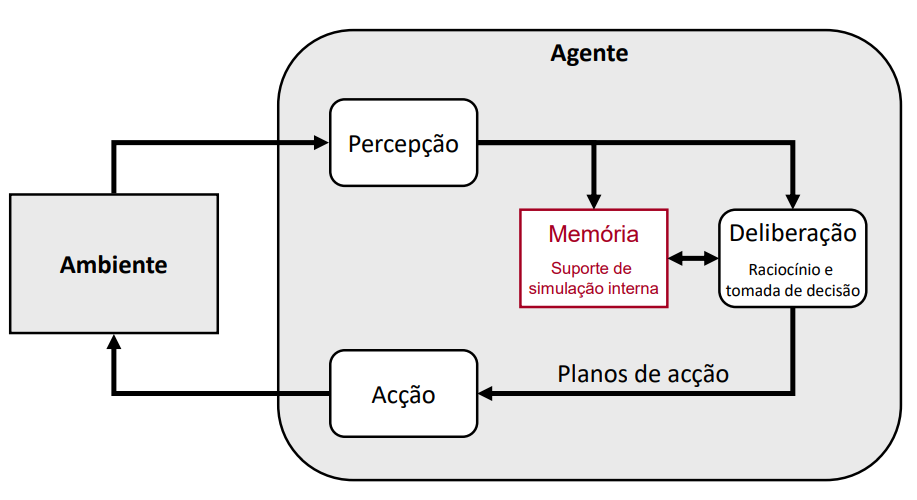
\includegraphics{../figures/arquitetura-deliberativa}}
    \end{center}
    \caption{Arquitetura deliberativa.
    Retirado de~\cite{isel:iasa:slides:arq-agentes-deliberativos}, slide 16.}
    \label{fig:arquitetura-deliberativa}
\end{figure}

É baseada em representações de conhecimento do domínio do problema, as quais
suportam a exploração de opções por simulação interna, para atingir objectivos
explicitamente representados, fixos ou gerados dinamicamente, tendo por base
processos de deliberação sobre que objectivos concretizar e quais os meios a utilizar

Numa arquitectura deliberativa o comportamento é gerado com base
em processos de planeamento suportados por representações internas
do ambiente (modelo do mundo)


\section{Implementação do Agente Deliberativo}\label{sec:implementacao-agente-deliberativo}
